\documentclass[../../main.tex]{subfiles}

\graphicspath{{\subfix{../../immagini/}}}

\begin{document}
    In questo paragrafo vengono presentati, e messi a confronto, i filtri appresi costruiti utilizzando le due tipologie di classificatore introdotte nel precedente paragrafo.

    Il primo aspetto su cui ragionare riguarda quale configurazione di iperparametri utilizzare per il percettrone: il classificatore migliore in questo caso non può essere trovato tramite una classica selezione del modello; nessuna metrica, infatti, risulta adatta a quantificare la bontà di un modello in termini di spazio occupato. Una model selection risulterebbe di conseguenza inadatta perché non avremmo nessuna metrica da massimizzare.

    Il numero di neuroni del percettrone viene quindi scelto in modo da ottenere un modello con una taglia molto vicina a quella della RNN con GRU a 16 dimensioni. Inoltre, dai risultati del precedente paragrafo è possibile notare come, aumentando di molto il numero di neuroni, l'aumento delle prestazioni non sia altrettanto significativo. Per questo motivo, viene considerato un ulteriore modello con un numero inferiore di neuroni al fine di evidenziare eventuali miglioramenti nello spazio occupato dai filtri appresi dovuti ad una dimensione minore del modello.

    Secondo questo ragionamento, viene considerata una configurazione con 30 neuroni, che ha una grandezza molto simile alla GRU 16, e una configurazione con 20 neuroni. In entrambi casi il learning rate viene fissato a 0.001, in quanto i risultati ottenuti nel precedente paragrafo suggeriscono che questa sia la scelta migliore.
    
    \paragraph{Scelta della soglia}
    Una volta scelti a priori il tasso di falsi positivi desiderato $f$ e il tasso di falsi positivi del classificatore, in questo paragrafo chiamato $f_{\tau}$, alla soglia $\tau$ viene assegnato un valore pari al quantile $100 \cdot (1 - f_{\tau})$ della distribuzione di valori predetti dal classificatore per le non-chiavi presenti nell'insieme d'addestramento.

    Coerentemente con quanto detto nel Paragrafo \ref{sec:falseProbLBF}, vengono considerati diversi valori di $\tau$ variando il valore del rapporto $r_{\tau} = f_{\tau}/f$. Si noti che, a seconda  del filtro considerato, dovranno valere le condizioni su $f_{\tau}$ descritte nel Capitolo \ref{chap:filtriAppresi}.

    \begin{table}[t]
        \centering
        \begin{tabular}{lcccc}
            \toprule
            {} & \multicolumn{4}{c}{\textbf{FPR $f$}}\\
            {} & 0.001 & 0.005 & 0.01 & 0.02\\
            \midrule
            \textbf{Dimensione (KByte)} & 76.774 & 58.887 & 51.212 & 43.479\\
            \bottomrule
        \end{tabular}
        \caption{Taglie dei filtri di Bloom per ogni tasso di falsi positivi $f$ considerato.}
        \label{tab:taglieFiltro}
    \end{table}

    \paragraph{Risultati del filtro di Bloom}

    Vengono riportate in Tabella \ref{tab:taglieFiltro} le taglie dei filtri di Bloom, inizializzati sull'insieme $\mathcal{K}$ delle chiavi, che verranno utilizzate come base per confrontare le performance dei filtri appresi riportate successivamente.

    Una volta fissato $f$, le taglie sono state calcolate secondo \eqref{eqn:nlowerbound}.

    \paragraph{Risultati LBF}
    Le \cref{fig:LBFFNRPercettrone,fig:LBFFPRPercettrone,fig:GRU_LBFFNR,fig:GRU_LBFFPR} mostrano graficamente i risultati delle analisi empiriche, al variare del rapporto $r_{\tau}$, effettuate sui filtri appresi costruiti con le due tipologie di classificatore (rete ricorrente e percettrone multistrato). Le Figure \ref{fig:tagliePercettroniLBF} e \ref{fig:taglieGRULBF}, invece, mostrano le taglie dell'intero LBF. In questo caso deve valere $0 < r_{\tau} < 1$, il rapporto viene quindi fatto variare tra questi due valori.

    Nello specifico, le Figure \ref{fig:LBFFNRPercettrone20} e \ref{fig:LBFFNRPercettrone30} per il percettrone, e \ref{fig:LBFFNR_GRU16}, \ref{fig:LBFFNR_GRU8} e \ref{fig:LBFFNR_GRU4} per la rete ricorrente, mostrano il tasso di falsi negativi prodotti dal classificatore al variare del rapporto $r_{\tau}$. Si nota in tutte le figure una diminuzione del rapporto di falsi negativi all'aumentare di $r_{\tau}$, ciò è sensato: all'aumentare di $r_{\tau}$ il valore della soglia $\tau$ diminuisce, di conseguenza è più probabile che una chiave venga classificata come tale, generando un numero di falsi negativi progressivamente minore.

    \begin{figure}[H]
        \centering
        \begin{subfigure}[b]{0.49\textwidth}
            \centering
            \includegraphics[width = \textwidth]{immagini/7/LBF/Percettrone(20, 0.001)_FNR.png}
            \caption{}
            \label{fig:LBFFNRPercettrone20}
        \end{subfigure}
        \begin{subfigure}[b]{0.49\textwidth}
            \centering
            \includegraphics[width = \textwidth]{immagini/7/LBF/Percettrone(30, 0.001)_FNR.png}
            \caption{}
            \label{fig:LBFFNRPercettrone30}
        \end{subfigure}
        \caption{Tasso di falsi negativi prodotti dall'LBF basato su percettrone. Il titolo di ogni grafico riporta la configurazione di iperparametri utilizzata, nella forma (Num. neuroni, Learning rate).}
        \label{fig:LBFFNRPercettrone}
    \end{figure}
    \begin{figure}[H]
        \begin{subfigure}[b]{0.49\textwidth}
            \centering
            \includegraphics[width = \textwidth]{immagini/7/LBF/Percettrone(20, 0.001)_FPR.png}
            \caption{}
            \label{fig:LBFFPRPercettrone20}
        \end{subfigure}
        \begin{subfigure}[b]{0.49\textwidth}
            \centering
            \includegraphics[width = \textwidth]{immagini/7/LBF/Percettrone(30, 0.001)_FPR.png}
            \caption{}
            \label{fig:LBFFPRPercettrone30}
        \end{subfigure}
        \caption{Tasso empirico di falsi positivi dell'LBF basato su percettrone. Il titolo di ogni grafico riporta la configurazione di iperparametri utilizzata, nella forma (Num. neuroni, Learning rate).}
        \label{fig:LBFFPRPercettrone}
    \end{figure}

    \begin{figure}[H]
        \centering
        \begin{subfigure}[b]{0.49\textwidth}
            \centering
            \includegraphics[width = \textwidth]{immagini/7/LBF/GRU16_FNR.png}
            \caption{}
            \label{fig:LBFFNR_GRU16}
        \end{subfigure}
        \begin{subfigure}[b]{0.49\textwidth}
            \centering
            \includegraphics[width = \textwidth]{immagini/7/LBF/GRU8_FNR.png}
            \caption{}
            \label{fig:LBFFNR_GRU8}
        \end{subfigure}
        \begin{subfigure}[b]{0.49\textwidth}
            \centering
            \includegraphics[width = \textwidth]{immagini/7/LBF/GRU4_FNR.png}
            \caption{}
            \label{fig:LBFFNR_GRU4}
        \end{subfigure}
        \caption{Tasso di falsi negativi prodotti dall'LBF basato su RNN. Il titolo di ogni grafico riporta la dimensione dello strato nascosto della GRU.}
        \label{fig:GRU_LBFFNR}
    \end{figure}
    \begin{figure}[H]
        \centering
        \begin{subfigure}[b]{0.49\textwidth}
            \centering
            \includegraphics[width = \textwidth]{immagini/7/LBF/GRU16_FPR.png}
            \caption{}
            \label{fig:LBFFPR_GRU16}
        \end{subfigure}
        \begin{subfigure}[b]{0.49\textwidth}
            \centering
            \includegraphics[width = \textwidth]{immagini/7/LBF/GRU8_FPR.png}
            \caption{}
            \label{fig:LBFFPR_GRU8}
        \end{subfigure}
        \begin{subfigure}[b]{0.49\textwidth}
            \centering
            \includegraphics[width = \textwidth]{immagini/7/LBF/GRU4_FPR.png}
            \caption{}
            \label{fig:LBFFPR_GRU4}
        \end{subfigure}
        \caption{Tasso empirico di falsi positivi dell'LBF basato su RNN. Il titolo di ogni grafico riporta la dimensione dello strato nascosto della GRU.}
        \label{fig:GRU_LBFFPR}
    \end{figure}

    Le \cref{fig:LBFFPRPercettrone20,fig:LBFFPRPercettrone30,fig:LBFFPR_GRU16,fig:LBFFPR_GRU8,fig:LBFFPR_GRU4}, invece, mostrano il tasso di falsi positivi $f$ dell'intero LBF, calcolato sull'insieme di test composto di soli URL legittimi. In questo caso, come previsto, il tasso empirico rimane sempre stabile attorno al tasso atteso.

    Infine, le \cref{fig:LBFTagliaPercettrone20,fig:LBFTagliaPercettrone30,fig:LBFTagliaGRU16,fig:LBFTagliaGRU8,fig:LBFTagliaGRU4} mostrano le taglie dei rispettivi classificatori al variare di $r_{\tau}$. Confrontando i risultati di percettrone e GRU si nota come, in tutti i casi, le due configurazioni di percettrone occupino uno spazio inferiore rispetto alle GRU. Inoltre, è facile notare che i filtri appresi con GRU non sono quasi mai migliori rispetto ai corrispettivi filtri di Bloom, al contrario, i percettroni sembrano occupare uno spazio minore rispetto ai relativi filtri. 

    Confrontando invece le taglie occupate dalle due configurazioni di percettrone, si nota come il modello a 20 neuroni sembri leggermente migliore rispetto a quello a 30. Questo conferma quanto supposto inizialmente: seppur il modello a 30 neuroni sia migliore in termini di performance, il modello con 20 neuroni risulta migliore se inserito all'interno di un filtro appreso. Le performance guadagnate dal percettrone a 30 neuroni non sono quindi sufficienti a giustificare l'aumento di spazio del modello.

    \begin{figure}[H]
        \centering
        \begin{subfigure}[b]{0.49\textwidth}
            \centering
            \includegraphics[width = \textwidth]{immagini/7/LBF/Percettrone(20, 0.001)_Taglia.png}
            \caption{}
            \label{fig:LBFTagliaPercettrone20}
        \end{subfigure}
        \begin{subfigure}[b]{0.49\textwidth}
            \centering
            \includegraphics[width = \textwidth]{immagini/7/LBF/Percettrone(30, 0.001)_Taglia.png}
            \caption{}
            \label{fig:LBFTagliaPercettrone30}
        \end{subfigure}
        \caption{Taglie $n$ dei LBF basati su percettrone. Il titolo di ogni grafico riporta la configurazione di iperparametri utilizzata, nella forma (Num. neuroni, Learning rate). Le rette tratteggiate rappresentano la taglia del relativo filtro di Bloom per il dato $f$.}
        \label{fig:tagliePercettroniLBF}
    \end{figure}

    \begin{figure}[H]
        \centering
        \begin{subfigure}[b]{0.49\textwidth}
            \centering
            \includegraphics[width = \textwidth]{immagini/7/LBF/GRU16_Taglia.png}
            \caption{}
            \label{fig:LBFTagliaGRU16}
        \end{subfigure}
        \begin{subfigure}[b]{0.49\textwidth}
            \centering
            \includegraphics[width = \textwidth]{immagini/7/LBF/GRU8_Taglia.png}
            \caption{}
            \label{fig:LBFTagliaGRU8}
        \end{subfigure}
        \begin{subfigure}[b]{0.49\textwidth}
            \centering
            \includegraphics[width = \textwidth]{immagini/7/LBF/GRU4_Taglia.png}
            \caption{}
            \label{fig:LBFTagliaGRU4}
        \end{subfigure}
        \caption{Taglie $n$ dei LBF basati su RNN. Il titolo di ogni grafico riporta la dimensione dello strato nascosto della GRU. Le rette tratteggiate rappresentano la taglia del relativo filtro di Bloom per il dato $f$.}
        \label{fig:taglieGRULBF}
    \end{figure}

    \paragraph{Risultati SLBF}
    Anche in questo caso, le \cref{fig:SLBFFNRPercettrone,fig:SLBFFPRPercettrone,fig:SLBFFNR_GRU,fig:SLBFFPR_GRU}  presentano i risultati empirici sulla performance dei filtri costruiti e le Figure \ref{fig:tagliePercettroniSLBF} e \ref{fig:taglieGRUSLBF}, invece, le rispettive taglie. In questo $r_{\tau}$ deve rispettare la condizione $(1 - m_b/m) \leq r_{\tau} \leq 1/f \cdot \left(1 - m_b/m\right)$.
    \begin{figure}[H]
        \centering
        \begin{subfigure}[b]{0.49\textwidth}
            \centering
            \includegraphics[width = \textwidth]{immagini/7/SLBF/Percettrone(20, 0.001)_FNR.png}
            \caption{}
            \label{fig:SLBFFNRPercettrone20}
        \end{subfigure}
        \begin{subfigure}[b]{0.49\textwidth}
            \centering
            \includegraphics[width = \textwidth]{immagini/7/SLBF/Percettrone(30, 0.001)_FNR.png}
            \caption{}
            \label{fig:SLBFFNRPercettrone30}
        \end{subfigure}
        \caption{Tasso di falsi negativi prodotti dall'SLBF basato su percettrone. Il titolo di ogni grafico riporta la configurazione di iperparametri utilizzata, nella forma (Num. neuroni, Learning rate).}
        \label{fig:SLBFFNRPercettrone}
    \end{figure}
    \begin{figure}[H]
        \begin{subfigure}[b]{0.49\textwidth}
            \centering
            \includegraphics[width = \textwidth]{immagini/7/SLBF/Percettrone(20, 0.001)_FPR.png}
            \caption{}
            \label{fig:SLBFFPRPercettrone20}
        \end{subfigure}
        \begin{subfigure}[b]{0.49\textwidth}
            \centering
            \includegraphics[width = \textwidth]{immagini/7/SLBF/Percettrone(30, 0.001)_FPR.png}
            \caption{}
            \label{fig:SLBFFPRPercettrone30}
        \end{subfigure}
        \caption{Tasso empirico di falsi positivi dell'SLBF basato su percettrone. Il titolo di ogni grafico riporta la configurazione di iperparametri utilizzata, nella forma (Num. neuroni, Learning rate).}
        \label{fig:SLBFFPRPercettrone}
    \end{figure}

    \begin{figure}[H]
        \centering
        \begin{subfigure}[b]{0.49\textwidth}
            \centering
            \includegraphics[width = \textwidth]{immagini/7/SLBF/GRU16_FNR.png}
            \caption{}
            \label{fig:SLBFFNR_GRU16}
        \end{subfigure}
        \begin{subfigure}[b]{0.49\textwidth}
            \centering
            \includegraphics[width = \textwidth]{immagini/7/SLBF/GRU8_FNR.png}
            \caption{}
            \label{fig:SLBFFNR_GRU8}
        \end{subfigure}
        \begin{subfigure}[b]{0.49\textwidth}
            \centering
            \includegraphics[width = \textwidth]{immagini/7/SLBF/GRU4_FNR.png}
            \caption{}
            \label{fig:SLBFFNR_GRU4}
        \end{subfigure}
        \caption{Tasso di falsi negativi prodotti dall'SLBF basato su RNN. Il titolo di ogni grafico riporta la dimensione dello strato nascosto della GRU.}
        \label{fig:SLBFFNR_GRU}
    \end{figure}
    \begin{figure}[H]
        \centering
        \begin{subfigure}[b]{0.49\textwidth}
            \centering
            \includegraphics[width = \textwidth]{immagini/7/SLBF/GRU16_FPR.png}
            \caption{}
            \label{fig:SLBFFPR_GRU16}
        \end{subfigure}
        \begin{subfigure}[b]{0.49\textwidth}
            \centering
            \includegraphics[width = \textwidth]{immagini/7/SLBF/GRU8_FPR.png}
            \caption{}
            \label{fig:SLBFFPR_GRU8}
        \end{subfigure}
        \begin{subfigure}[b]{0.49\textwidth}
            \centering
            \includegraphics[width = \textwidth]{immagini/7/SLBF/GRU4_FPR.png}
            \caption{}
            \label{fig:SLBFFPR_GRU4}
        \end{subfigure}
        \caption{Tasso empirico di falsi positivi dell'SLBF basato su RNN. Il titolo di ogni grafico riporta la dimensione dello strato nascosto della GRU.}
        \label{fig:SLBFFPR_GRU}
    \end{figure}

    Il ragionamento già fatto per gli LBF può essere ripetuto anche in questo caso: il tasso di falsi negativi del classificatore diminuisce all'aumentare di $r_{\tau}$, e il tasso di falsi positivi empirico è sempre molto vicino a quello atteso.

    Nelle \cref{fig:SLBFFNRPercettrone20,fig:SLBFFNRPercettrone30,fig:SLBFFNR_GRU16,fig:SLBFFNR_GRU8,fig:SLBFFNR_GRU4} si nota però una differenza rispetto ai risultati precedenti: per ogni $f$ il tasso di falsi negativi raggiunge in questo caso valori più bassi rispetto ai relativi LBF, in alcuni casi arrivando quasi a zero. Questo accade a causa di valori di $f_\tau$ testati più alti, che portano a valori di $\tau$ più bassi.

    Il tasso di falsi negativi molto basso è utile a spiegare l'andamento dei grafici \cref{fig:SLBFTagliaPercettrone20,fig:SLBFTagliaPercettrone30,fig:SLBFTagliaGRU16,fig:SLBFTagliaGRU8,fig:SLBFTagliaGRU4}, che mostrano come variano le dimensioni dei filtri al variare di $r_\tau$. Nella Figura \ref{fig:SLBFTagliaPercettrone20}, ad esempio, l'andamento della curva relativa a $f = 0.02$ è crescente, e ciò è giustificabile ricordando come vengono calcolate le taglie $n_{b_0}$ e $n_b$ (si veda \eqref{eqn:SLBFGrandezzaOttimaInit} e \eqref{eqn:SLBFGrandezzaOttima}). Se il numero di falsi negativi $m_b$ tende a 0, allora anche la grandezza del filtro di backup $n_b$ tenderà a 0; viceversa, la taglia del filtro $n_{b_0}$ continuerà a crescere, generando l'andamento crescente evidenziato dalla figura.

    Anche in questo caso, confrontando le Figure \ref{fig:tagliePercettroniSLBF} e \ref{fig:taglieGRUSLBF}, sembra che il percettrone risulti migliore per ogni $f$ testato. Si noti però che, in questo caso, anche la GRU fornisce prestazioni migliori in termini di spazio rispetto al filtro base.

    \begin{figure}[H]
        \centering
        \begin{subfigure}[b]{0.49\textwidth}
            \centering
            \includegraphics[width = \textwidth]{immagini/7/SLBF/Percettrone(20, 0.001)_Taglia.png}
            \caption{}
            \label{fig:SLBFTagliaPercettrone20}
        \end{subfigure}
        \begin{subfigure}[b]{0.49\textwidth}
            \centering
            \includegraphics[width = \textwidth]{immagini/7/SLBF/Percettrone(30, 0.001)_Taglia.png}
            \caption{}
            \label{fig:SLBFTagliaPercettrone30}
        \end{subfigure}
        \caption{Taglie $n$ dei SLBF basati su percettrone. Il titolo di ogni grafico riporta la configurazione di iperparametri utilizzata, nella forma (Num. neuroni, Learning rate). Le rette tratteggiate rappresentano la taglia del relativo filtro di Bloom per il dato $f$.}
        \label{fig:tagliePercettroniSLBF}
    \end{figure}

    \begin{figure}[H]
        \centering
        \begin{subfigure}[b]{0.49\textwidth}
            \centering
            \includegraphics[width = \textwidth]{immagini/7/SLBF/GRU16_Taglia.png}
            \caption{}
            \label{fig:SLBFTagliaGRU16}
        \end{subfigure}
        \begin{subfigure}[b]{0.49\textwidth}
            \centering
            \includegraphics[width = \textwidth]{immagini/7/SLBF/GRU8_Taglia.png}
            \caption{}
            \label{fig:SLBFTagliaGRU8}
        \end{subfigure}
        \begin{subfigure}[b]{0.49\textwidth}
            \centering
            \includegraphics[width = \textwidth]{immagini/7/SLBF/GRU4_Taglia.png}
            \caption{}
            \label{fig:SLBFTagliaGRU4}
        \end{subfigure}
        \caption{Taglie $n$ dei SLBF basati su RNN. Il titolo di ogni grafico riporta la dimensione dello strato nascosto della GRU. Le rette tratteggiate rappresentano la taglia del relativo filtro di Bloom per il dato $f$.}
        \label{fig:taglieGRUSLBF}
    \end{figure}

    \paragraph{Confronto con la codifica binaria}
    Vengono ora presentati i risultati ottenuti utilizzando la codifica binaria presentata nel Paragrafo \ref{sec:implementazione}. Da alcuni esperimenti è emerso che addestrare il percettrone utilizzando questa codifica porta, a parità di iperparametri, a delle performance migliori. 
    
    Il problema principale deriva dal fatto che, utilizzando questa tipologia di codifica, la dimensione dei vettori in ingresso aumenta notevolmente, aumentando di conseguenza la taglia del modello. Nel nostro dataset, ad esempio, la codifica con CountVectorizer porta a vettori di dimensione 82, mentre usando questa la codifica binaria (troncata a 30 caratteri), i vettori hanno dimensione 210. Per ovviare a questo problema la soluzione è ridurre il numero di neuroni nascosti, riducendo di conseguenza il numero totale di parametri del modello.

    Le Figure \ref{fig:tagliePercettroniBinLBF} e \ref{fig:tagliePercettroniBinSLBF} mostrano le taglie dei filtri ottenuti utilizzando la codifica binaria e 8 neuroni per lo strato nascosto, portando ad un numero totale di parametri simile a quello del modello a 20 neuroni.

    \begin{figure}[H]
        \centering
        \begin{subfigure}[b]{0.48\textwidth}
            \centering
            \includegraphics[width=\textwidth]{immagini/7/LBF/Percettrone(8, 0.001) Binario_Taglia.png}
            \caption{}
        \end{subfigure}
        \begin{subfigure}[b]{0.48\textwidth}
            \centering
            \includegraphics[width=\textwidth]{immagini/7/LBF/Percettrone(20, 0.001)_Taglia.png}
            \caption{}
        \end{subfigure}
        \caption{Confronto con la codifica binaria. Vengono riportate le taglie $n$ dei LBF basati su percettrone. Il titolo di ogni grafico riporta la configurazione di iperparametri utilizzata, nella forma (Num. neuroni, Learning rate). Le rette tratteggiate rappresentano la taglia del relativo filtro di Bloom per il dato $f$.}
        \label{fig:tagliePercettroniBinLBF}
    \end{figure}

    \begin{figure}[H]
        \centering
        \begin{subfigure}[b]{0.48\textwidth}
            \centering
            \includegraphics[width=\textwidth]{immagini/7/SLBF/Percettrone(8, 0.001) Binario_Taglia.png}
            \caption{}
        \end{subfigure}
        \begin{subfigure}[b]{0.48\textwidth}
            \centering
            \includegraphics[width=\textwidth]{immagini/7/SLBF/Percettrone(20, 0.001)_Taglia.png}
            \caption{}  
        \end{subfigure}
        \caption{Confronto con la codifica binaria. Vengono riportate le taglie $n$ dei SLBF basati su percettrone. Il titolo di ogni grafico riporta la configurazione di iperparametri utilizzata, nella forma (Num. neuroni, Learning rate). Le rette tratteggiate rappresentano la taglia del relativo filtro di Bloom per il dato $f$.}
        \label{fig:tagliePercettroniBinSLBF}
    \end{figure}

    Seppur il percettrone binario abbia performance migliori rispetto alle RNN presentate, il percettrone con la codifica utilizzata fino ad ora risulta comunque migliore. Per questo motivo nei confronti successivi verranno riportati solamente i risultati relativi codifica CountVectorizer.

    \paragraph{Confronto tra filtri di Bloom, LBF e SLBF}
    Le Tabelle \ref{tab:confrontoFinaleLBF} e \ref{tab:confrontoFinaleSLBF} mettono a confronto le taglie rispettivamente di LBF e SLBF nel caso migliore. In entrambe le tipologie di filtro il percettrone a 20 neuroni risulta essere la scelta migliore. Inoltre, per ogni $f$ testato, l'SLBF fornisce un miglioramento più ampio rispetto al relativo LBF.
    
    Infine, la Figura \ref{fig:ConfrontoFinale} mostra a livello grafico lo stesso confronto presentato dalle due tabelle.
    \begin{table}[H]
        \centering
        \begin{tabular}{llcccc}
            \toprule
            {} & {}  & \multicolumn{4}{c}{\textbf{FPR $f$}}\\
            {} & {}  & 0.001 & 0.005 & 0.01 & 0.02\\
            \midrule
            \multicolumn{6}{c}{\textbf{Filtro di Bloom}}\\
            \midrule
            {} & $n$ & 76.774 & 58.887 & 51.212 & 43.479\\
            \midrule 
            \multicolumn{6}{c}{\textbf{LBF}}\\
            \midrule
            \multirow{2}{*}{\textbf{Perc. (20, 0.001)}} & $n$ &  \cellcolor{red!25}67.881 & \cellcolor{red!25}40.821 & \cellcolor{red!25}29.649 & \cellcolor{red!25}20.554\\
            & $n_c$ & 6.809 &  6.809 &  6.809 &  6.809 \\
            \hdashline 
            \multirow{2}{*}{\textbf{Perc. (30, 0.001)}} & $n$ & 68.420 & 41.536 & 30.983 & 22.581\\
            & $n_c$ & 10.090 & 10.090 & 10.090 & 10.090\\   
            \hdashline 
            \multirow{2}{*}{\textbf{GRU 16}} & $n$ & 85.676 & 66.307 & 52.265 & 35.646\\
            & $n_c$ & 9.671 &  9.671 &  9.671 &  9.671\\
            \hdashline 
            \multirow{2}{*}{\textbf{GRU 8}}& $n$ & 79.955 & 60.030 & 49.810 & 40.047\\
            & $n_c$&  6.701 &  6.701 &  6.701 &  6.701\\
            \hdashline 
            \multirow{2}{*}{\textbf{GRU 4}}& $n$ & 80.557 & 62.734 & 54.656 & 45.309\\
            & $n_c$ &  5.779 &  5.779 &  5.779 &  5.779\\ 
            \bottomrule
        \end{tabular}
        \caption{Confronto delle taglie degli LBF nel caso migliore. Vengono evidenziate le celle corrispondenti alla taglia più bassa. Tutte le taglie riportate sono in KByte. La notazione $n_c$ indica la taglia del classificatore.}
        \label{tab:confrontoFinaleLBF}
    \end{table}

    \begin{table}[H]
        \centering
        \begin{tabular}{llcccc}
            \toprule
            {} & {}  & \multicolumn{4}{c}{\textbf{FPR $f$}}\\
            {} & {}  & 0.001 & 0.005 & 0.01 & 0.02\\
            \midrule
            \multicolumn{6}{c}{\textbf{Filtro di Bloom}}\\
            \midrule
            {} & $n$ & 76.774 & 58.887 & 51.212 & 43.479\\
            \midrule 
            \multicolumn{6}{c}{\textbf{SLBF}}\\
            \midrule           
            \multirow{4}{*}{\textbf{Perc. (20, 0.001)}} & $n$ & \cellcolor{red!25}54.585  & \cellcolor{red!25}35.823 & \cellcolor{red!25}28.119 & \cellcolor{red!25}20.415\\
            & $n_{b_0}$ & 29.575 & 17.746 & 10.042 &  2.338\\
            & $n_{b}$ & 18.201 & 11.268 & 11.268 & 11.268\\
            & $n_c$ &  6.809 &  6.809 &  6.809 &  6.809\\
            \hdashline 
            \multirow{4}{*}{\textbf{Perc. (30, 0.001)}} & $n$ & 55.981 & 37.953 & 30.325 & 22.622\\
            & $n_{b_0}$ & 29.096 & 14.870 &  9.799 &  2.095\\
            & $n_{b}$ & 16.795 & 12.993 & 10.436 & 10.436\\
            & $n_c$ & 10.090 & 10.090 & 10.090 & 10.090\\
            \hdashline 
            \multirow{4}{*}{\textbf{GRU 16}} & $n$   & 71.822 & 46.744 & 39.086 & 31.411\\
            & $n_{b_0}$ & 34.894 & 26.986 & 20.203 & 10.584\\
            & $n_{b}$ & 27.258 & 10.087 &  9.212 & 11.155\\
            & $n_c$ &  9.671 &  9.671 &  9.671 &  9.671\\
            \hdashline 
            \multirow{4}{*}{\textbf{GRU 8}} & $n$  & 72.834 & 44.386 & 36.040 & 28.443\\
            & $n_{b_0}$ & 37.367 & 28.068 & 23.094 & 14.082\\
            & $n_{b}$ & 28.765 &  9.617 &  6.245 &  7.660\\
            & $n_c$ &  6.701 &  6.701 &  6.701 &  6.701\\
            \hdashline 
            \multirow{4}{*}{\textbf{GRU 4}} & $n$  & 77.271 & 52.095 & 40.479 & 30.176\\
            & $n_{b_0}$ & 42.709 & 31.346 & 27.628 & 22.101\\
            & $n_{b}$ & 28.782 & 14.970 &  7.073 &  2.296\\
            & $n_c$ &  5.779 &  5.779 &  5.779 &  5.779\\
            \bottomrule          
        \end{tabular}
        \caption{Confronto delle taglie degli SLBF nel caso migliore. Vengono evidenziate le celle corrispondenti alla taglia più bassa. Tutte le taglie riportate sono in KByte. La notazione $n_c$ indica la taglia del classificatore.}
        \label{tab:confrontoFinaleSLBF}
        \end{table}

        \begin{figure}[H]
            \centering
            \begin{subfigure}[b]{0.48\textwidth}
                \centering
                \includegraphics[width=\textwidth]{immagini/7/LBF/Confronto.png}
                \label{fig:LBFConfrontoFinale}
                \caption{}
            \end{subfigure}
            \begin{subfigure}[b]{0.48\textwidth}
                \centering
                \includegraphics[width=\textwidth]{immagini/7/SLBF/Confronto.png}
                \label{fig:SLBFConfrontoFinale}
                \caption{}
            \end{subfigure}
            \caption{Confronto delle taglie nel caso migliore per ogni $f$ testato: (a) nel caso di un LBF (b) nel caso di un SLBF.}
            \label{fig:ConfrontoFinale}
        \end{figure}

    \paragraph{Tempi di accesso}
    Un ultimo aspetto importante da considerare è il tempo di accesso per ognuna delle tipologie di filtro proposte. Le Tabelle \ref{tab:tempiMediLBF} e \ref{tab:tempiMediSLBF} mostrano i tempi medi d'accesso per elemento, rispettivamente per LBF ed SLBF.

    Dalle tabelle emerge che il filtro di Bloom classico risulta più veloce di circa 1-2 ordini di grandezza, a seconda del classificatore considerato, rispetto alle controparti apprese. La minore efficienza in termini di tempo dei filtri appresi è molto probabilmente dovuta alla maggiore complessità della struttura: nel filtro di Bloom, infatti, l'accesso consiste semplicemente nel calcolo delle funzioni di hash, mentre nelle strutture apprese è necessario anche interrogare il classificatore per ottenere i valori delle predizioni; più un classificatore è complesso, maggiore sarà il tempo necessario per questa operazione. Questo viene anche confermato dal fatto che i filtri che utilizzano la GRU 16 sono quelli con il tempo medio di accesso più alto.

    \begin{table}[H]
        \centering
        \begin{tabular}{lrrrr}
            \toprule
            & \multicolumn{4}{c}{\textbf{FPR} $f$}\\
            & 0.001 & 0.005 & 0.10 & 0.20\\        
            \midrule
            \textbf{Filtro di Bloom} & 9.976E-07 & 1.06E-06 & 9.41E-07 & 7.94E-07\\
            \midrule
            \textbf{Perc. (20, 0.001)} & 8.843E-06 & 8.814E-06 &  8.774E-06 & 8.770E-06\\
            \textbf{Perc. (30, 0.001)} & 8.848E-06 & 8.869E-06 &  8.826E-06 & 8.764E-06\\
            \textbf{GRU 16} & 4.546E-05 & 4.545E-05 &  4.540E-05 & 4.542E-05\\
            \textbf{GRU 8} &  2.180E-05 & 2.173E-05 &  2.174E-05 & 2.171E-05\\
            \textbf{GRU 4} & 1.519E-05 & 1.516E-05 & 1.513E-05 & 1.511E-05\\
            \bottomrule
        \end{tabular}
        \caption{Tempi di accesso medi per elemento su LBF(calcolati su 5 iterazioni).}
        \label{tab:tempiMediLBF}
    \end{table}

    \begin{table}[H]
        \centering
        \begin{tabular}{lrrrr}
            \toprule
            & \multicolumn{4}{c}{\textbf{FPR} $f$}\\
            & 0.001 & 0.005 & 0.10 & 0.20\\        
            \midrule
            \textbf{Filtro di Bloom} & 9.976E-07 & 1.06E-06 & 9.41E-07 & 7.94E-07\\
            \midrule
            \textbf{Perc. (20, 0.001)} & 8.085E-06 & 8.189E-06 &  8.258E-06 & 8.203E-06\\
            \textbf{Perc. (30, 0.001)} & 8.135E-06 & 8.171E-06 &  8.231E-06 & 8.127E-06\\
            \textbf{GRU 16} & 4.542E-05 & 4.552E-05 &  4.555E-05 & 4.555E-05\\
            \textbf{GRU 8} &  1.972E-05 & 1.981E-05 &  1.985E-05 & 1.987E-05\\
            \textbf{GRU 4} & 1.454E-05 & 1.464E-05 & 1.471E-05 & 1.471E-05\\
            \bottomrule
        \end{tabular}
        \caption{Tempi di accesso medi per elemento su SLBF(calcolati su 5 iterazioni).}
        \label{tab:tempiMediSLBF}
    \end{table}

    In ultimo, è interessante notare che, nonostante il filtro aggiuntivo, i tempi dei SLBF siano simili e, in alcuni casi, leggermente migliori rispetto a quelli dei relativi LBF. Dato che l'SLBF comprende un filtro iniziale, il numero di chiamate al classificatore è minore rispetto a un LBF, questo potrebbe giustificare i tempi più bassi della struttura a sandwich.
\end{document}